\documentclass[border=10pt]{standalone}
\usepackage{tikz}
\usetikzlibrary{arrows.meta, calc, patterns}

\begin{document}

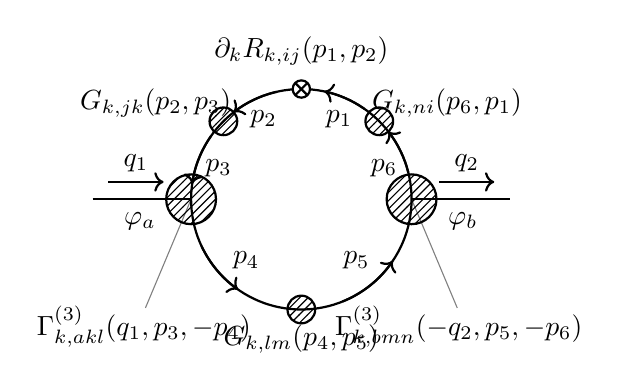
\begin{tikzpicture}[scale=1, every node/.style={scale=1}, >=To]
    \def\R{1.4}

    % External legs
    \draw[thick] (-2.65,0) -- (-\R,0);
    \draw[thick] (\R,0) -- (2.65,0);
    \draw[->, thick] (-2.45,0.22) -- node[above] {$q_1$} (-1.75,0.22);
    \draw[->, thick] (1.75,0.22) -- node[above] {$q_2$} (2.45,0.22);
    \node at (-2.05,-0.28) {$\varphi_a$};
    \node at (2.05,-0.28) {$\varphi_b$};

    % Thin grey leader lines for the three-point vertices
    \draw[gray, thin] (-1.98,-1.38) -- (-\R,0);
    \draw[gray, thin] (1.98,-1.38) -- (\R,0);

    % Central propagator loop
    \draw[thick] (0,0) circle (\R);
    \draw[->, thick] ({\R*cos(55)},{\R*sin(55)}) arc[start angle=55,end angle=78,radius=\R];
    \draw[->, thick] ({\R*cos(103)},{\R*sin(103)}) arc[start angle=103,end angle=128,radius=\R];
    \draw[->, thick] ({\R*cos(145)},{\R*sin(145)}) arc[start angle=145,end angle=172,radius=\R];
    \draw[->, thick] ({\R*cos(205)},{\R*sin(205)}) arc[start angle=205,end angle=235,radius=\R];
    \draw[->, thick] ({\R*cos(292)},{\R*sin(292)}) arc[start angle=292,end angle=326,radius=\R];
    \draw[->, thick] ({\R*cos(14)},{\R*sin(14)}) arc[start angle=14,end angle=38,radius=\R];

    % Dressed vertices on the loop and external attachments
    \node[circle, draw, thick, fill=white, pattern=north east lines, minimum size=10pt, inner sep=0pt] at ({\R*cos(135)},{\R*sin(135)}) {};
    \node[circle, draw, thick, fill=white, pattern=north east lines, minimum size=10pt, inner sep=0pt] at ({\R*cos(45)},{\R*sin(45)}) {};
    \node[circle, draw, thick, fill=white, pattern=north east lines, minimum size=10pt, inner sep=0pt] at (0,-\R) {};
    \node[circle, draw, thick, fill=white, pattern=north east lines, minimum size=18pt, inner sep=0pt] at (-\R,0) {};
    \node[circle, draw, thick, fill=white, pattern=north east lines, minimum size=18pt, inner sep=0pt] at (\R,0) {};

    % Regulator insertion at the top of the loop
    \draw[thick, fill=white] (0,\R) circle (0.11);
    \draw[thick] (-0.075,{\R-0.075}) -- (0.075,{\R+0.075});
    \draw[thick] (-0.075,{\R+0.075}) -- (0.075,{\R-0.075});

    % Momentum labels on the circular loop
    \node at (0.48,1.02) {$p_1$};
    \node at (-0.48,1.02) {$p_2$};
    \node at (-1.05,0.40) {$p_3$};
    \node at (-0.70,-0.78) {$p_4$};
    \node at (0.70,-0.78) {$p_5$};
    \node at (1.05,0.40) {$p_6$};

    % Mathematical notations
    \node at (0,1.88) {$\partial_k R_{k,ij}(p_1,p_2)$};
    \node at (-1.85,1.22) {$G_{k,jk}(p_2,p_3)$};
    \node at (1.85,1.22) {$G_{k,ni}(p_6,p_1)$};
    \node at (-2.0,-1.62) {$\Gamma_{k,akl}^{(3)}(q_1,p_3,-p_4)$};
    \node at (2.0,-1.62) {$\Gamma_{k,bmn}^{(3)}(-q_2,p_5,-p_6)$};
    \node at (0,-1.77) {$G_{k,lm}(p_4,p_5)$};

\end{tikzpicture}

\end{document}
